% Masterthesis
%
% Multiscale Modelling Group of Jun.-Prof. Birgit Strodel
%
% Author:
% Oliver Schillinger


\ifdefined\isdraft
    \documentclass[english, a4paper, 12pt, titlepage, draft]{article}
\else
    \documentclass[english, a4paper, 12pt, titlepage, final]{article}
\fi

\usepackage{geometry}
\usepackage[british]{babel}
\usepackage{graphicx,hyperref,url,color,cite}
\usepackage[table]{xcolor}
\usepackage{mathtools}
\usepackage[latin1]{inputenc}

\definecolor{fzjblue50}{cmyk}{1,0.2,0.05,0.50}
\definecolor{fzjblue35}{cmyk}{1,0.2,0.05,0.35}
\definecolor{fzjblue30}{cmyk}{1,0.2,0.05,0.30}
\definecolor{fzjblue20}{cmyk}{1,0.2,0.05,0.20}
\definecolor{fzjblue10}{cmyk}{1,0.2,0.05,0.10}
\definecolor{fzjgray80}{cmyk}{0,0,0,0.8}
\definecolor{fzjgray50}{cmyk}{0,0,0,0.5}
\definecolor{fzjgray30}{cmyk}{0,0,0,0.3}

\usepackage{framed}
\definecolor{shadecolor}{cmyk}{1,0.2,0.05,0.10}

\usepackage{mdframed}
\mdfsetup{
    framemethod=tikz,
    linewidth=10pt,
    linecolor=fzjblue50,
%    innerlinewidth=10pt,
%    middlelinewidth=10pt,
%    outerlinewidth=10pt,
%    innerlinecolor=red,
%    middlelinecolor=green,
%    outerlinecolor=blue,
    backgroundcolor=fzjgray30,
    roundcorner=15pt}
%\newmdenv[linecolor=black,backgroundcolor=fzjblue10,roundcorner=10pt,linewidth=5pt]{titlebox}
%\newmdenv[linecolor=red]{titlebox}

\usepackage{setspace}
\usepackage[version=3]{mhchem}

\hypersetup{
    %bookmarks=false,                      % show bookmarks bar?
    unicode=true,                          % non-Latin characters in Acrobat’s bookmarks
    pdftoolbar=true,                       % show Acrobat’s toolbar?
    pdfmenubar=true,                       % show Acrobat’s menu?
    pdffitwindow=false,                    % window fit to page when opened
    pdfstartview={FitH},                   % fits the width of the page to the window
    pdftitle={Masterthesis},               % title
    pdfauthor={Oliver Schillinger},
    pdfsubject={Masterthesis},             % subject of the document
    pdfcreator={Oliver Schillinger},       % creator of the document
    pdfproducer={Oliver Schillinger},      % producer of the document
    pdfkeywords={Lipase} {CitA} {GROMACS}, % list of keywords
    pdfnewwindow=true,                     % links in new window
    colorlinks=true,                       % false: boxed links; true: colored links
    linkcolor=black,                       % color of internal links
    citecolor=blue,                        % color of links to bibliography
    filecolor=red,                         % color of file links
    urlcolor=cyan                          % color of external links
}

\newcommand{\PDB}[1]{\href{http://pdb.rcsb.org/pdb/explore/explore.do?structureId=#1}{#1}}

% Formula typesetting commands
\newcommand{\vect}[1]{\mathbf{#1}}
\newcommand{\norm}[1]{\left\Vert#1\right\Vert}
\newcommand{\fun}[2]{#1\left(#2\right)} 
\newcommand{\vfun}[2]{\vect{#1}\left(#2\right)} 
\newcommand{\vfunv}[2]{\vect{#1}\left(\vect{#2}\right)} 

% Figure template
%\begin{figure}
%    \centering
%    \includegraphics[width=0.5\textwidth]{figures/draft/draft.pdf}
%    \caption{}
%    \label{fig:}
%\end{figure} 


% ============================================================================ %


\begin{document}

% ============================================================================ %

\begin{titlepage}
\begin{center}
{\huge \textbf{Masterthesis}}\\
\vspace{2cm}

{\textbf{Registered Title:} \\
Elucidating the structure of a fusion protein of a lipase and a citrate binding domain by Molecular Dynamics simulation
}

\vspace{2cm}
%\begin{shaded*}
%\begin{titlebox}
\begin{mdframed}
    \centering
{\large \textbf{Protein Structure and Dynamics} \\
\vspace{1cm}
of \textit{Bacillus Subtilis} Lipase LipA Fused to the Ligand-Binding Domain of Sensor Histidine Kinase CitA
}
\end{mdframed}
%\end{titlebox}
%\end{shaded*}

\vspace{2cm}

Oliver Schillinger \\
Forschungszentrum J\"ulich \\ Institute of Complex Systems 6 - Structural Biochemistry \\ Multiscale Modelling Group \\
Supervisor: Jun.-Prof. Dr. Birgit Strodel \\
\vspace{1cm}
German Research School for Simulation Sciences \\
RWTH Aachen

\vspace{1cm}

\today

\vfill

\begin{figure}[h!]
\includegraphics[width=.3\textwidth]{figures/logos/grs_logo.pdf}
\hspace{0.5cm}
\includegraphics[width=.3\textwidth]{figures/logos/fzj_logo.pdf}
\hspace{0.5cm}
\includegraphics[width=.3\textwidth]{figures/logos/rwth_logo.pdf}
\end{figure}
 
\end{center}
\end{titlepage}


% ============================================================================ %

\onehalfspacing

\begin{abstract}

A fusion protein of the periplasmic domain of sensor histidine kinase CitA from \textit{Klebsiella Pneumoniae} and the lipase LipA from \textit{Bacillus Subtilis} is investigated by means of molecular dynamics simulation.
The research was motivated by experiments indicating that CitA's natural ligand citrate down-regulates lipase activity upon binding.
Both proteins were first studied independently.
It was found that the citrate binding pocket was stable in the citrate bound crystal structure when studied in a 100 ns molecular dynamics simulation after careful equilibration.
The unfused, solo lipase was also very stable during a simulation of the same length, especially the binding pocket and the catalytic residues maintained their relative conformations.
As no crystal structure of the fusion protein is known, several possible structures have been generated \emph{in silico} by Basin Hopping.
The fusion protein showed dynamics that differ significantly from those of the isolated proteins.
The presence of citrate in the receptor binding pocket did not stabilize the structure to the same extend compared to the isolated CitA.
The presence of a covalently bound citrate binding domain to the lipase destabilized the LipA binding pocket significantly.
This is most likely the reason for the experimentally found activity degradation in lipase activity.

\end{abstract}


% ============================================================================ %

\pagenumbering{roman}
\tableofcontents

\pagebreak

\onehalfspacing

\pagenumbering{arabic}

% ============================================================================ %

\section{Introduction}

The structure and kinetics of two proteins under investigation are well known:
The periplasmic domain of sensor \textit{Klebsiella Pneumoniae} histidine kinase CitA (CitAP, PDB accession code \PDB{2J80}) \cite{CitA_2J80}
and the lipase LipA of \textit{Bacillus Subtilis} (BSLA, PDB accession code \PDB{1I6W}), \cite{BSLA_1I6W} both in their ligand bound and ligand free states.
CitAP is a periplasmic citrate receptor that, upon activation by citrate binding, triggers a cytoplasmic reaction cascade starting with the autophosphorylation of the endoplasmic domain of CitA and finally leading to the transcription of citrate fermentation genes.
%BSLA's efficient lipid hydrolysis capability is industrially utilized for many applications, including its use as an additive in laundry detergents.
What is not understood is the structure and kinetics of a fusion protein of these two peptides.
It was hypothesized that citrate binding could influence lipase activity, thus creating a switchable detergent.
Activity measurements indicate that citrate binding to the sensor kinase domain indeed down-regulates lipase activity (Figure \ref{fig:BSLAactivity}).
This effect is of major interest to the chemical industry as lipases exhibit a wide diversity in substrate specificity and have found applications in the resolution of racemic mixtures, the synthesis of esters, transesterification reactions and as additives in laundry detergents.
As chemical applications would benefit from the opposite effect, a controlled up-regulation of lipase activity triggered by citrate addition, this research focused on the structure elucidation of the fused protein, as well as on the mechanism by which lipase activity is regulated.
A thorough understanding of this mechanism might in the future enable us to engineer the protein to invert the regulatory effect of citrate binding.
The main methods used for structure elucidation are global optimization using the combined Monte Carlo -- energy minimization approach Basin Hopping, followed by high-throughput molecular dynamics simulations. 
 

\begin{figure}
    \centering
    \includegraphics[width=0.5\textwidth]{figures/BSLA_activity/BSLA_activity.png}
    \caption{The activity of the BSLA--CitAP complex is reduced after citrate addition while the uncomplexed lipase is not affected.
    EC50 indicates the concentration of ligand that causes a half-maximal effect (here: change in lipolytic activity)
    Experiments performed by Karl Erich Jaeger et al., data unpublished.}   
    \label{fig:BSLAactivity}
\end{figure}


% ============================================================================ %

\section{Proteins Under Investigation}

% ==================================== %

\subsection{\textit{Bacillus Subtilis} Lipase LipA}

\textit{Bacillus Subtilis} is a gram-positive, aerobic bacterium found in soil and water that is subject to active research since 1992 \cite{bacillusSubtilis}.
\textit{Bacillus Subtilis} is of major industrial interest because of its highly efficient protein secretion system \cite{BSsecretion}, enabling the production of proteases and amylases in bulk quantities \cite{BSworkhorse}.
Of special interest are its excreted lipases, as these catalyze the hydrolysis and synthesis of long chain triacylglycerols \cite{BSLA_1I6W}.
These lipases possess a wide substrate specificity.
They find applications in transesterification reactions, the synthesis of esters, the resolution of racemic mixtures and are used as additives in laundry detergents \cite{BSdetergents}.

The reported experiments where performed using lipase LipA from \textit{Bacillus Subtilis} (BSLA).
Compared to lipases from other organisms BSLA is relatively small, consisting of 181 amino acids and weighing 19.36 kDA.
BSLA belongs to the $\alpha$-$\beta$ hydrolase fold enzymes.
Members of this protein family are constituted by a twisted $\beta$-strand core flanked by alpha helices on both sides \cite{alphaBetaHydrolases}.
Because of its small size and because other known $\alpha$-$\beta$ hydrolase fold enzymes extend on this core structure, it can be considered a minimal $\alpha$-$\beta$ hydrolase.
BSLA hydrolyses sn-1 and sn-3 glycerol esters with long fatty acid chains, while its highest activity is exhibited on medium sized fatty acids \cite{BSLA_1I6W}.
The optimum environment is reported to be found at pH 10 \cite{BSLA_1I6W}.

Most known lipases possess an $\alpha$-helical segment that covers the active site.
The encounter of lipid-aggregates triggers the opening of this lid, exposing the active site and triggering catalytic activity.
This behaviour is known as interfacial activation \cite{alphaBetaHydrolases}.
BSLA lacks this lid, resulting in an active site that is solvent exposed and thus actively hydrolysing fatty acids even in the absence of lipid-aggregates.

The active site is located at the bottom of a shallow cleft formed by four turns (Figure \ref{fig:BSLAactiveSite}).
Its structure is in accordance with the secondary structure topology of the canonical $\alpha$/$\beta$-hydrolase fold, in which the active site is formed by a nucleophile, an acid and a histidine, together called the catalytic triad \cite{BSLA_1I6W}.
In BSLA this catalytic triad is constituted of Serine 77 (nucleophile), Aspartate 133 (acid) and Histidine 156.
Serine 77 is located at the so called nucleophilic elbow \cite{nucleophileElbow}, a sharp turn at the bottom of the binding pocket connecting a central $beta$-sheet to a peripheral $\alpha$-helix.
The ester hydrolysis catalyzed by BSLA is depicted in Figure \ref{fig:BSLAreaction}.
The ligand binds covalently with its phosphoryl group to Serine 77.
A tetrahedral intermediate structure is formed.
The phosphoryl oxygen of the substrate is hydrogen bound to the \ce{NH} atoms of Methionine 78 and Isoleucine 12, forming the oxyanion hole that is common to most lipases \cite{BSLA_1I6W}.
The \ce{N^{$\epsilon$}} atom of His156 is located at hydrogen bonding distance from the Ser77 \ce{O^{$\gamma$}} atom and the substrate ester oxygen.






\begin{figure}
    \centering
    \includegraphics[width=0.8\textwidth]{figures/BSLA_pocket/BSLA_pocket_cartoon.pdf}
    \caption{Active site of \textit{Bacillus Subtilis} lipase LipA with Sc-IPG-phosphonate-inhibitor bound.
    The catalytic triad residues are colored, as well as the backbone nitrogen atoms forming the oxyanion hole.
    Coordinates taken from PDB accession code \PDB{1R50}.}
    \label{fig:BSLAactiveSite}
\end{figure} 

\begin{figure}
    \centering
    \includegraphics[width=0.7\textwidth]{figures/BSLA_reaction.png}
    \caption{Ester hydrolysis reaction catalyzed by BSLA. Taken from \cite{BSLA_reaction}.}
    \label{fig:BSLAreaction}
\end{figure}  





% ==================================== %

\subsection{Periplasmic Domain of Sensor Histidine Kinase CitA}

CitA is the sensor histidine kinase of a two component regulatory (TCR) system of \textit{Klebsiella Pneumoniae} \cite{CitA_original}.
TCR systems generally consist of a sensor histidine kinase and a response regulator (CitB in the present case).
Sensor histidine kinases respond to environmental conditions by autophosphorylation of a conserved histidine residue.
The phosphoryl group is subsequently transferred to a conserved Aspartate residue on the response regulator.
The phosphorylated response regulator in turn triggers a change in gene expression or cell behaviour \cite{CitA_original}.
The CitA/CitB regulatory system controls the expression of citrate fermentation genes.
Citrate metabolism requires careful regulation, as an uncontrolled transcription of citrate fermentation genes in the absence of citrate would break the citric acid cycle with severe consequences for the organism \cite{CitA_original}.

Like most known sensor histidine kinases, CitA is a membrane protein, the domain composition of which is shown in Figure \ref{fig:CitA_organization}.
Its extracellular N-terminal sensor domain is flanked by two transmembrane helices, one of which links to the intracellular autokinase domain.
Like virtually all known sensor histidine kinases, CitA appears to be dimeric \cite{2CST}.
In many cases only the structures of extracellular domains of sensor kinases are known, due to the inherent difficulties of obtaining structural information about membrane proteins.
This is also true for CitA, where only structures of the periplasmic domain (CitAP) have been resolved.
CitAP consists of 135 amino acid residues, weighing a total of 14.68 kDA.

The overall fold of the periplasmic domain of sensor histidine kinases classifies them as members of the Per-Arnt-Sim domain superfamily.
This superfamily comprises many well studied sensor histidine kinases \cite{PAS}.


\begin{figure}
    \centering
    \includegraphics[width=0.7\textwidth]{figures/CitA_organization.png}
    \caption{CitA domain organization. Only the structure of the periplasmic domain (CitAP) is known and was used in the reported research. Histidine 350 gets phosphorylated after signal transduction as described in the text. Figure taken from \cite{CitA_original}}
    \label{fig:CitA_organization}
\end{figure}   


The mechanism of action of CitA \cite{CitA_original} is initiated by citrate binding, triggering a conformational change of the periplasmic domain that is mediated by a transmembrane helix to the cytoplasmic kinase domain.
It has been hypothesized that this mediation happens by a piston-like mechanism (Figure \ref{fig:CitA_mechanism}) in which transmembrane helix 2 is pulled to the periplasmic side of the membrane.
The resulting conformational change in the kinase domain allows the interaction of the ATP-binding subdomain with the cytoplasmic phosphorylation subdomain.
After autophosphorylation the subdomains dissociate.
The phosphorylation subdomain can now bind to the receiver domain of the response regulator CitB.
A final phosphotransfer in the phosphorylation domain from histidine to an Aspartate completes the CitA cycle and a new response can be triggered.


\begin{figure}
    \centering
    \includegraphics[width=0.7\textwidth]{figures/CitA_mechanism.png}
    \caption{Hypothetical mode of action of CitA. The citrate-triggered conformational change of the periplasmic domain is mediated to the cytoplasmic kinase domain by a piston-like mechanism. Figure taken from \cite{CitA_2J80}}
    \label{fig:CitA_mechanism}
\end{figure}    



The binding pocket of CitAP is build up from a $\beta$-sheet core that forms the bottom and two loops, the minor loop (residue 96 to 106) and the major loop (residue 63 to 92).
These loops form tight lids covering the bound ligand and forming a closed pocket.
While the \textit{in vivo} conformation of the termini remains uncertain due to crystal packing artifacts, the core structure of the bound CitAP has been solved with 1.6 $\mathring{A}$ resolution and has been experimentally found to be well folded in solution \cite{CitA_2J80}.
The major loop is unresolved in the unbound CitAP structures, indicating that it is highly mobile without the stabilizing effect of the ligand.
The core structure of the protein is highly similar for the bound and unbound structures with similar backbone positions and sidechain orientations of the binding residues not located in the minor or major loop \cite{CitA_2J80}.

A sodium ion attached to the first helix and the $\beta$-sheet core has been crystallized in the citrate bound structures.
Its physiological significance had already been indicated, as sodium is required for the induction of the CitA/CitB target genes \cite{KlebsiellaMetabolism} and is backed by the by the fact that no sodium has been found in the citrate free crystal structure.

It has been reported that citrate binding to CitAP is highly specific and that virtually all CitAP is in the bound state under physiological citrate concentrations \cite{CitA_2J80}.
Citrate interacts mainly with Thr58, Arg66, His69, Glu80, Ser101, Leu102, Arg107, Lys109 and Ser124 by hydrogen bonding (Figure \ref{fig:citrate_interactions}).
A further hydrogen bond is mediated by a water molecule to Gly103.
The conformational change in the periplasmic domain of sensor histidine kinase CitA is illustrated in Figure \ref{fig:CitA_opening}.
The main conformational change is a flattening of the $\beta$-sheet that forms the minor loop.
Upon citrate binding this $\beta$-sheet is pulled in, due to interaction with the ligand.
This disrupts some of the interactions with neighbouring $\beta$-sheets and subsequently pulls the C-terminus away from the membrane.
The unstructured major loop in the citrate free crystal structure indicates that the citrate binding pocket is less stable in absence of citrate.


\begin{figure}
    \centering
    \includegraphics[width=0.7\textwidth]{figures/CitAP_conf_change/CitAP_conf_change.pdf}
    \caption{The conformational change in the periplasmic domain of sensor histidine kinase CitA.
    The minor loop flexes from the bound conformation (blue) to the open conformation (red).
    Citrate bound and free coordinates have been taken from PDB structures \PDB{2J80} and \PDB{2R50} respectively.
    The major loop (green) is only present in the bound structure as it was indicated to be unstructured in the ligand free form, at least under crystallization conditions.}
    \label{fig:CitA_opening}
\end{figure}     



\begin{figure}
    \centering
    \includegraphics[width=0.7\textwidth]{figures/citrate_interactions/citrate_interactions.pdf}
    \caption{Interactions of CitAP with its bound ligand citrate as determined by visual inspection of a 1ns molecular dynamics trajectory. The minor loop is the domain with the largest RMSD in the transition from citrate bound to citrate free conformation.}
    \label{fig:citrate_interactions}
\end{figure}      


% ==================================== %

\subsection{Fusion Complex}

The two proteins described earlier have been fused in the laboratory, motivated by the desire to regulate the lipolytic activity of BSLA.
A controlled up regulation by a cheap and non-toxic molecule such as citrate could be utilized to switch on the desired catalysis at specified times.
It was assumed that the conformational change of CitAP triggered by citrate binding could have a regulatory effect on lipase activity.
Experiments have been performed by Jaeger et al. to test this hypothesis (Figure \ref{fig:BSLAactivity}).

The sequence of the fused construct, as used in the experiments performed in the group of Karl-Erich Jaeger, is shown in Figure \ref{fig:complex_sequence}.
CitAP was connected to BSLA by means of a linker helix that was taken from YtvA, the blue light sensor of \textit{Bacillus Subtilis} (PDB accession code: \PDB{2PR5}).
A polyhistidine-tag (His-tag) was attached to allow easy purification and
an Xa protease site was included in the complexed protein as it was found experimentally that this increased the effect of citrate on BSLA activity.
The construct consists of 336 amino acid residues and weighs 36.21 kDA.

Although it was attempted to up-regulate the lipase activity by citrate binding, experiments indicated the opposite effect (Figure \ref{fig:BSLAactivity}).
While increasing citrate concentrations had no effect on the activity of uncomplexed BSLA, lipolysis was significantly reduced at higher citrate concentrations in the CitAP--BSLA complex protein to about 40\% of the initial activity of the complex.

Jaeger et al. determined by sedimentation velocity analytical ultracentrifugation, that the fusion protein exists mainly as a monomer with globular shape (results not published).




\begin{figure}
    \centering
    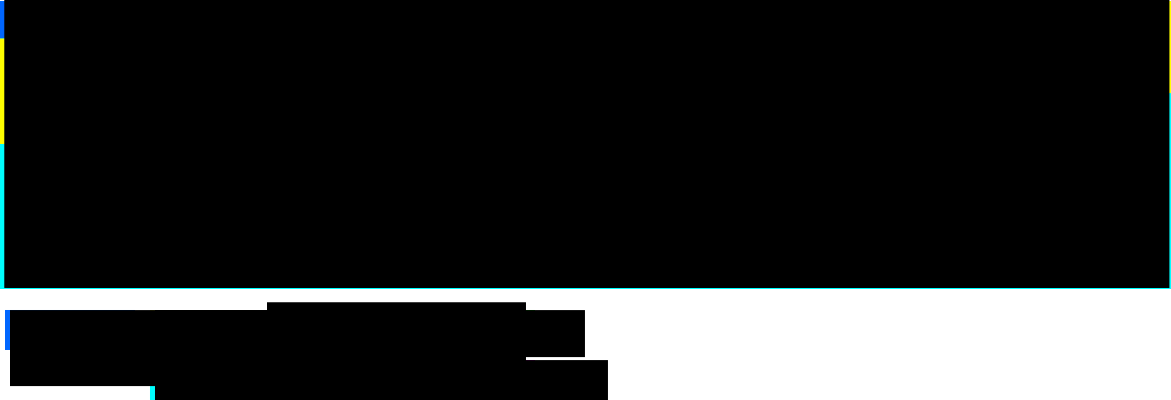
\includegraphics[width=0.9\textwidth]{figures/Complex_sequence/Complex_sequence.pdf}
    \caption{Amino acid sequence of the BSLA--CitAP complex. The coordinates of amino acids represented in bold font have been taken from the respective PDB coordinate files.
    The remaining amino acids are present in the construct that was used in experiments performed in the group of Professor Jaeger. These amino acids have been modelled into the \emph{in silico} structure of the fusion protein.}
    \label{fig:complex_sequence}
\end{figure}       


% ============================================================================ %

\section{Methods}
\subsection{Molecular Dynamics}

The main method that was used in the presented research is Molecular Dynamics simulations (MD) based on classical Molecular Mechanics (MM) \cite{MDintro}.
In Molecular Mechanics, molecules are modelled as systems of chemically inert atoms that interact through Newtonian mechanics.
The interaction energy between atoms is described by preferably simple mathematical equations, mainly harmonic and trigonometric functions, as well as the well known electrostatic and Lennard-Jones potentials.
A given set of potential energy formulas, together with its parameters, is called a force field, as it is used to compute the interatomic forces (see also section \ref{sec:forcefields}).
This chapter describes the theory of the various sub-algorithms that are relevant for molecular dynamics simulations.


\subsubsection{Integrators}

Newtons equations of motion are numerically integrated to obtain a trajectory in phase-space.
A naive approach would be to use a simple Euler integration scheme \cite{Euler} using the Taylor expansion of the particle positions truncated after the second order term:

\begin{equation}
    \vfun{r}{t+\Delta t} = \vfun{r}{t} + \vfun{v}{t}\Delta t + \frac{\vfun{f}{t}}{2m} \Delta t^2 + \mathcal{O}(\Delta t^3),
    \label{eq:Euler}
\end{equation} 

 where $\vect{v}$ and $\vect{f}$ represent the particle velocities and forces respectively and $m$ is the particle mass. 
For simplicity all particles are assumed to be of equal mass here.
The velocity update in the Euler method is computed as:

\begin{equation}
    \vfun{v}{t+\Delta t} = \vfun{v}{t} + \frac{\vfun{f}{t}}{2m} \Delta t+ + \mathcal{O}(\Delta t^2)
\end{equation}

Although this algorithm might seem reasonably simple first, it turns out to be a particularly bad choice as it is irreversible and suffers from an inherent energy shift \cite{FrenkelSmit}.
Several different integration schemes have been introduced over the years.
It is easiest to start the discussion with the Verlet algorithm \cite{Verlet}.
This algorithm is based on two Taylor expansions of the particle position, forward and backward in time:

\begin{equation}
    \vfun{r}{t+\Delta t} = \vfun{r}{t} + \vfun{v}{t}\Delta t + \frac{\vfun{f}{t}}{2m} \Delta t^2 + \frac{\Delta t^3}{3!} \vfun{\dddot r}{t} + \fun{\mathcal{O}}{\Delta t^4}
    \label{eq:Verlet1}
\end{equation}

and

\begin{equation}
    \vfun{r}{t-\Delta t} = \vfun{r}{t} - \vfun{v}{t}\Delta t + \frac{\vfun{f}{t}}{2m} \Delta t^2 - \frac{\Delta t^3}{3!} \vfun{\dddot r}{t} + \fun{\mathcal{O}}{\Delta t^4}.
    \label{eq:Verlet2}
\end{equation} 

Summing equations \ref{eq:Verlet1} and \ref{eq:Verlet2} and solving for $\vfun{r}{t+\Delta t}$ yields the position update relation of the Verlet integrator:

\begin{equation}
    \vfun{r}{t+\Delta t} = 2\vfun{r}{t} - \vfun{r}{t-\Delta t} + \frac{\vfun{f}{t}}{m} \Delta t^2 + \mathcal{O}(\Delta t^4)
    \label{eq:VerletPos}
\end{equation}

It is interesting to note, that the Verlet algorithm computes the position update from the positions at the two preceding time steps, bypassing the computation of the velocities altogether.
As the velocities are essential for an estimate of the kinetic energy and hence the temperature, they might still be computed as

\begin{equation}
    \vfun{v}{t} = \frac{\vfun{r}{t-\Delta t} - \vfun{r}{t+\Delta t}}{2\Delta t} + \mathcal{O}(\Delta t^2),
\end{equation}

but only up to an accuracy of order $\mathcal{O}(\Delta t^2)$.
The Verlet algorithm also suffers from the fact that it needs two subsequent initial time steps to start the integration procedure and define the velocities.

Integration schemes exist, that are equivalent to the Verlet integration in the sense that they give rise to the same (analytical) trajectories, but yield a higher accuracy for the velocity computation and the corresponding evaluations of kinetic energy and temperature.
The Leap Frog integration algorithm starts out by subtracting the Taylor expansions of equations \ref{eq:Verlet1} and \ref{eq:Verlet2}, rather than summing them up, and truncating after the third order term, therefore initially losing an order of accuracy right from the start:

\begin{equation}
    \vfun{v}{t} = \frac{\vfun{r}{t+\Delta t} - \vfun{r}{t-\Delta t}}{2 \Delta t} + \mathcal{O}(\Delta t^3)
    \label{eq:LeapFrog1}
\end{equation}

Shifting the result by $+\Delta t$ and dividing the time step by $2$ gives:

\begin{equation}
    \vfun{v}{t + \Delta t/2} = \frac{\vfun{r}{t+\Delta t} - \vfun{r}{t}}{\Delta t} + \mathcal{O}(\Delta t^3)
    \label{eq:LeapFrogShift1}
\end{equation}

Shifting equation \ref{eq:LeapFrog1} instead in opposite direction results in:

\begin{equation}
    \vfun{v}{t - \Delta t/2} = \frac{\vfun{r}{t} - \vfun{r}{t-\Delta t}}{\Delta t} + \mathcal{O}(\Delta t^3)
    \label{eq:LeapFrogShift2}
\end{equation} 

The last equation gives a direct way of updating the positions:

\begin{equation}
    \vfun{r}{t+\Delta t} = \vfun{r}{t} + \Delta t \vfun{v}{t+\Delta t/2} + \mathcal{O}(\Delta t^3)
\end{equation}

To get a relation for the velocity update, equations \ref{eq:LeapFrogShift1} and \ref{eq:LeapFrogShift2} need to be subtracted and combined with equation \ref{eq:VerletPos}:

\begin{equation}
    \vfun{v}{t+\Delta t/2} = \vfun{v}{t-\Delta t/2} + \Delta t \frac{\vfun{f}{t}}{m} + \mathcal{O}(\Delta t^3)
\end{equation}

One order of accuracy for the velocity computation has been gained at the cost of one order of accuracy for the position update compared to the Verlet integration.
An additional disadvantage of this method is the fact that position and velocities are not computed at the same, but rather at alternating half-integer time steps.
This complicates the evaluation of potential, kinetic and total energy, as these are as well not defined at the same time.
It is however possible to get rid of this additional problem by casting the Verlet algorithm in a different form, known as the velocity Verlet algorithm.
Its equation for the position update is the same as in the Euler integrator.
To arrive at the velocity update relation of the velocity Verlet algorithm we start out by adding both sides of the relation for the Verlet position update (equation \ref{eq:VerletPos}) shifted by $+\Delta t$ to the naive Euler position update relation (equation \ref{eq:Euler}).
Rearranging and collecting like terms gives:

\begin{equation}
    \vfun{r}{t+2\Delta t} - \vfun{r}{t+\Delta t} = \Delta t \vfun{v}{t} + \frac{\Delta t^2}{2m} \left[ 2\vfun{f}{t+\Delta t} + \vfun{f}{t} \right] + \mathcal{O}(\Delta t^3)
\end{equation}

Insertion of the $\Delta t$-shifted Euler position update relation into the last equation and solving for $\vfun{v}{t+\Delta t}$ results in:

\begin{equation}
    \vfun{v}{t+\Delta t} = \vfun{v}{t} + \frac{\Delta t}{2m} \left[ \vfun{f}{t+\Delta t} + \vfun{f}{t}\right]  + \mathcal{O}(\Delta t^3)
\end{equation}

The velocity Verlet algorithm is therefore able to compute the velocity and the positions at the same integer time steps, while maintaining the same order of accuracy as the Leap Frog algorithm.
In case this accuracy is high enough, the velocity Verlet algorithm is the best choice among the presented algorithms, the only problem being that its implementation in the latest version of the molecular dynamics package GROMACS does not support all temperature and pressure control mechanisms.

% ==================================== %

\subsubsection{Force Fields}
\label{sec:forcefields}

An exact calculation of the behaviour of a molecular system involves solving the Schr\"odinger equation for all electrons and nuclei.
As the computaional complexity for this problem grows extremely fast with increasing system size, the direct solution of all but the smallest molecular system is infeasible.
Parameterized, analytical descriptions have been developed for a simplified description of interatomic interactions in and between molecules that enable simulations of large molecular systems.
The mathematical form of these equations is inspired by knowledge of the physics and chemistry that govern molecular interactions.
The parameters are chosen to reproduce energy functions of quantum mechanical descriptions of model systems.
As the large number of parameters, the choice of the model systems and the quantum chemical methods used for reference computations are all degrees of freedom in the paremterization, several different sets of parameters exist.
A set of equations with its corresponding parameters is called a force field.
This section first discusses the mathematical form of relatively simple, non polarizable force fields and then gives reasons for the choice of a particular implementation.

\paragraph{Lennard-Jones Potential}
A simple but often reasonable model of atomic structure treats atoms as nuclei surrounded by a diffuse electron cloud.
Some elements possess a permanent dipole moment due to the shape and occupation of their electronic orbitals.
Three kind of interactions between electron clouds give rise to the Van-der-Waals interaction, which is one contribution to the Lennard-Jones potential.
First, two permanent dipoles interact and will attract or repel each other depending on their mutual alignment.
The second contribution to the Van-der-Waals interaction comes from dipoles induced in the electron cloud by permanent dipoles of neighbouring atoms.
This interaction is attractive, as the induced dipole will have the same polarization as the inducing dipole due to repelling electron clouds.
Finally, the electron clouds of two unpolarized atoms repel each other, therefore inducing dipoles that in turn give rise to a dipole--dipole interaction.
The sum of these 3 effects is the source of the Van-der-Waals interaction and gives rise to an overall attractive force that decays with the sixth square root of the inter atomic distance.

Two atoms that approach each other will be affected by the Pauli exclusion principle that prohibits electrons from having the same state.
This prevents two atoms to occupy the same space and will result in a repelling force at close distances.
This and the dipole interactions of the electron clouds together are cast in the Lennard Jones potential that contains a term for short range repulsion and one for long range attraction (Figure \ref{fig:LJ} and equation \ref{eq:LJ}).
For each pair of elements a force field needs to specify two parameters to define their equilibrium distance and the depth of the interaction well.
Many force fields list only one set of parameters per element and give a relation for the computation of parameters for the Lennard-Jones interaction of two different elements.
The Lennard-Jones interaction converges fast to a constant value, and with it the resulting force goes to zero.
This fast convergence makes a truncation at a suitable cutoff distance possible.
However, for an accurate computation of the potential energy, the constant term at this cutoff distance needs to be accounted for.

\begin{figure}
    \begin{minipage}[]{0.45\linewidth}
        \centering
        \vfill
        \begin{equation}
            V_{LJ}(r_{ij}) = \frac{C^{(12)}_{ij}}{r^{12}_{ij}} - \frac{C^{(6)}_{ij}}{r^{6}_{ij}}
            \label{eq:LJ}
        \end{equation} 
        \vfill 
    \end{minipage}
\hspace{0.5cm}
    \begin{minipage}[]{0.45\linewidth}
        \centering
        \includegraphics[width=\textwidth]{figures/Argon_dimer_potential.png} 
    \end{minipage}
    \caption{Left: Lennard-Jones potential formula ($C^{*}_{ij}$ are the coefficients to be parameterized and $r_{ij}$ is the inter atomic distance). Right: Argon dimer potential. Source: \url{http://en.wikipedia.org/wiki/File:Argon_dimer_potential.png}}
\label{fig:LJ}
\end{figure}


\paragraph{Coulomb potential}
The computation of the coulomb interaction (equation \ref{eq:CoulombPot}, $q_i$ is the charge on atom $i$ and $\epsilon_0$ is the dielectric constant of vacuum) is particularly tricky as the electrostatic force decays slowly with increasing distance and suffers from ill convergence.
This problem is treated with sophisticated methods for long range electrostatic interactions as described in section \ref{sec:PME}.
The partial charges on each atom that are needed for the evaluation of the coulomb potential are also part of the force field parameter set and are usually derived from quantum chemical calculations.

\begin{equation}
    V_C(r_{ij}) = \frac{1}{4\pi \epsilon_0} \frac{q_i q_j}{r_{ij}}
    \label{eq:CoulombPot}
\end{equation}

\paragraph{Bonded Forces}
Apart from the non-bonded inter atomic forces there also exist interaction potentials due to bonds between the atoms of a molecule.
Bond stretching (equation \ref{eq:bonded}), bond angle bending (equation \ref{eq:angle}), proper and improper dihedral angles (equations \ref{eq:dihedral} and \ref{eq:improper} respectively) can all be modelled by harmonic potentials, but more sophisticated mathematical forms exist as well.
Bond stretching is defined by an equilibrium distance between two atom types $r^0_{ij}$ and an interaction constant $k^b_{ij}$.
Bond angles are parameterized by an equilibrium angle between three atom types and a constant ($\theta^0_{ijk}$, $k^a_{ijk}$).
Dihedral and improper dihedral angles depend on interaction constants and equilibrium angles between planes spanned by three atoms $ijk$ and $jkl$ ($\phi^0_{ijkl}$, $\xi^0_{ijkl}$, $k^d_{ijkl}$ and $k^{id}_{ijkl}$).


\begin{eqnarray}
    V_b(r_{ij})        & = & \frac{1}{2} k^b_{ij}(r_{ij}-r^0_{ij})^2 \label{eq:bonded} \\
    V_a(\theta_{ijk})  & = & \frac{1}{2} k^a_{ijk}(\theta_{ijk}-\theta^0_{ijk})^2 \label{eq:angle} \\
    V_d(\phi_{ijkl})   & = & k^d_{ijkl}(1+cos(n\phi_{ijkl}-\phi^0_{ijkl})) \label{eq:dihedral}\\
    V_{id}(\xi_{ijkl}) & = & \frac{1}{2} k^{id}_{ijkl}(\xi_{ijkl}-\xi^0_{ijkl})^2 \label{eq:improper}
\end{eqnarray}




The described potentials are only the simplest to use in molecular force fields ant a variety of others exist that result in more accurate representations, especially for the dihedral angles.
A great variety of force fields exists and a careful and well informed choice about the set of equations and parameters that can model the system under investigation best has to be made.
Recent benchmarks of protein force fields give insights into the strengths and weaknesses of the available options \cite{proteinFF}, indicating that one of the most up to date corrections to the widely used amber force field (\texttt{amber99sb-ildn-nmr}) \cite{amber99sb-ildn-nmr} is the best choice for simulations of proteins in explicit solvent.
For the cited benchmark a statistical evaluation of the performance of various force fields compared to real experiments was performed.
A number of di- and tripeptides served as model systems for chemical shift measurements in NMR experiments.
The deviations of the measurements from chemical shifts, computed on the basis of molecular dynamics trajectories performed with the investigated force fields, are reported.
In general, older force field parameterization sets performed worse than newer corrections for all force fields studied.
The chosen correction to the \texttt{amber99} force field performed best in simulations of ubiquitin, the only full length protein studied in the benchmark.
This led to the decision to use this force field for the reported experiments.

% ==================================== %

\subsubsection{Citrate Parameterization}

The \texttt{amber99sb-ildn-nmr} force field parameterizes only amino and nucleic acids, biologically relevant ions, water and a very limited set of other molecules.
It does not include parameters for citrate.
Force field parameters for use with the amber force fields were generated with the tool ACPYPE \cite{ACPYPE}.
ACPYPE acts as an interface to the Antechamber programs from the Ambertools package \cite{antechamber}.
In particular, it uses the general amber force field (GAFF) \cite{GAFF} to generate topologies for small organic molecules that can directly be used with GROMACS in combination with one of the amber force fields.
GAFF is an empirical approach to force field parameterization for arbitrary molecules.
It inherits the Van-der-Waals parameters from the \texttt{amber99} force fields directly.
Parameters for the bonded interactions have been fitted to \textit{ab initio} calculations and equilibrium bond length and angles have also been estimated by real experiments.
A crucial point in topology generation with GAFF is the assignment of partial charges.
Ideally, this should be done based on elaborate quantum chemical calculations.
There exist however other means of empirical partial charge assignments.
The charges assigned to citrate for this research have been estimated with the AM1-BCC model \cite{am1bcc_method} \cite{am1bcc_validation}.
This model tries to generate charges that emulate the electrostatic potential of \textit{ab initio} Hartree Fock calculations with the HF/6-31G* basis set.


% ==================================== %

\subsubsection{Long--Range Electrostatics}
\label{sec:PME}

The electrostatic potential decays relatively slowly with increasing distance (equation \ref{eq:CoulombPot}).
As a result, the computation of electrostatic interactions converges slowly and cannot simply be cut off at a specified distance without introducing significant artifacts \cite{FrenkelSmit}.
Efficient techniques have been developed to arrive at and accurate and, at the same time, fast computation of the electrostatic energy in periodic systems.
The problem to be solved is the estimation of a solution to Poisson's equation:

\begin{equation}
    -\nabla^2 \phi(\vect{r}) = 4 \pi \rho(\vect{r}),
\end{equation}

where $\phi$ is the electrostatic potential and $\rho$ is the charge density function.
Gaussian units are used.

All approaches to tackle long range electrostatics efficiently rely either on multipole expansions or on summations in reciprocal space that converge much faster than the corresponding sums in direct space.
The starting point is to split the electrostatic interaction into an easily computable short range and a harder to estimate long range part:

\begin{equation}
    \phi(\vect{r}) = \phi_{sr}(\vect{r}) + \phi_{lr}(\vect{r})
\end{equation}

The short range part is evaluated directly by a sum over all atoms up to the short range cutoff distance.
The long range part is then computed in reciprocal space by Fourier transforming the charge distribution, performing the evaluation of the fast converging reciprocal electrostatic interaction function and back transforming the result to direct space.
The straight forward implementation of this is known as Ewald summation, invented by P.P. Ewald in 1921 \cite{Ewald}.
The Ewald method has a complexity of $\mathcal{O}(n^{3/2})$ and scales therefore only to limited system sizes.

A method that scales a lot better, at the order of $\mathcal{O}(n \cdot log(n))$, is the Particle-Mesh-Ewald method (PME) \cite{PME}.
Instead of Fourier transforming the long range part of the electrostatic interaction directly, the charges are assigned to the nodes of a grid covering the direct space.
The grid can then be transformed to reciprocal space utilizing the fast Fourier transform algorithm (FFT), which itself scales as $\mathcal{O}(n \cdot log(n))$.
After evaluation of the interaction in reciprocal space, the inverse FFT transforms the result back to direct space.
This techniques enables efficient treatment of long range interactions that scales well to large system sizes.
In the GROMACS MD package, the FFT is done in parallel on a designated number of processors to limit communication to a minimum.



% ==================================== %

\subsubsection{Temperature \& Pressure Control}
\label{sec:tempPressControl}

According to the ergodic hypothesis, a histogram of states visited by a thermodynamical system during an infinite time span equals a histogram of an infinite number of copies of the same system in thermodynamical equilibrium at one instant of time.
In other words, averages of system properties over time will equal averages over states in phase space.
These distributions of states at thermodynamic equilibrium are summarized in the concept of ensembles \cite{Atkins}. 
Each of a number of possible ensembles (i.e. distributions of states) is associated with system properties that are constant for all states of that ensemble.
The thermodynamic ensemble that is produced by a molecular dynamics simulation is controlled by the macroscopic properties that are kept constant during the simulation
The ensemble directly affects the behaviour of the system and therefore the measured quantities.
A naive approach to molecular simulation would keep the number of particles ($N$), the system volume ($V$) and the total energy of the system ($E$) constant, as this does not require any control of extensive, and thus hard to influence quantities.
This will yield distributions from the microcanonical, or $NVE$ ensemble, which does not correspond to any situation that is easy to create in a laboratory.
Two other ensembles result in distributions that are much more directly comparable to real world experiment.
The canonical, or $NVT$ ensemble, requires a proper control of temperature (T) and reflects experimental conditions of constant volume and constant temperature.
The grand canonical ensemble, or $NPT$ ensemble, needs an additional mechanism to control the pressure (P).
$NPT$ is the desired ensemble for most biomolecular simulations, as it corresponds directly to \textit{in vivo} situations, where the pressure and temperature are controlled by the environment and in general thought to remain constant on chemically relevant time scales.

Several algorithms exist for pressure control during MD simulations.
The Berendsen algorithm (\cite{BerendsenTempControl}) rescales the velocities in order to match the differential equation

\begin{equation}
    \frac{dT}{dt} = \frac{T_0 - T}{\tau},
\end{equation}

that couples the system exponentially with a time constant $\tau$ to a heat bath of temperature $T_0$.
The Berendsen thermostat suppresses fluctuations of kinetic energy and therefore does not generate a proper thermodynamic ensemble. It might still be used for equilibration purposes.

The Nose-Hoover thermostat (\cite{Nose}, \cite{Hoover}) extends the system Hamiltonian by coupling to a thermal reservoir with a friction term $\xi$.
The reservoir has its own momentum $p_{\xi}$, a mass-like parameter $Q$ and follows its own dynamic equations of motion:

\begin{equation}
    \frac{dp_{\xi}}{dt} = (T-T_0),
\end{equation}

coupling the reservoir momentum to a reference temperature $T_0$.
The new equation of motion for the particles is:

\begin{equation}
    \frac{d^2\vect{r}_i}{dt^2} = \frac{\vect{F}_i}{m_i} - \frac{p_{\xi}}{Q} \frac{d\vect{r}_i}{dt}
\end{equation}

The Nose-Hoover thermostat can be extended to couple the heat reservoir to another bath, which in turn couples to a further bath and so forth to generate a chain of baths.
This Nose-Hoover chain is guaranteed to be ergodic in the limit of infinite chain length.
The system temperature under control of a Nose-Hoover chain will oscillate around a reference value and it is therefore not suited for equilibration if the system starts out at a totally different temperature.

A third temperature control algorithm is the velocity rescaling thermostat, which, as the name suggests, rescales the velocities similar to the Berendsen thermostat with the improvement of an additional stochastic term that ensures the generation of a proper thermodynamic ensemble distribution.

Pressure control happens along the same lines of the algorithms outlined for temperature control.
A Berendsen analog for pressure coupling exists and the Parinello-Rahman (\cite{ParrinelloRahman}) and Martyna-Tuckerman-Tobias-Klein (MTTK, \cite{MTTK}) algorithms are similar in spirit to the Nose-Hoover thermostat, coupling the pressure to a pressure bath.
One additional complication of pressure control is the definition and computation of the pressure in a bulk system.
It is defined with the virial equation:

\begin{equation}
    PV = Nk_BT + \frac{1}{D} \left< \sum^N_{i=1}\vect{r}_i \vect{F}_i \right>
\end{equation}

The virial equation relates the pressure to the average over the forces acting on all particles.
The pressure computed in this way is a highly fluctuating quantity and only its average can be meaningfully interpreted.

% ==================================== %

\subsubsection{Water Model}

Despite being a small and at first sight simple molecule, the properties of water are particularly hard to model properly.
This is mainly due to the complex interactions between water molecules that form complicated networks, especially in the liquid phase.
A wide range of models have been invented, some of which get close to reality in the prediction of water properties like density, dipole moment, dielectric constant and the self diffusion, but none of them can be regarded as perfect as each has its own shortcomings.
A detailed overview of water models is given at \url{http://www.lsbu.ac.uk/water/models.html}.
Water models can be distinguished by the geometry that they adapt to model real water.
Planar models exist that either place all partial charges on the atoms themselves (e.g. SPC and tip3p water models), or introduce a virtual interaction site on which a partial charge is deposited (e.g. tip4p water model).
This latter was introduced to improve the prediction of the dipole moment.
More elaborate models are of tetrahedral shape with partial charges pointing in the direction of the oxygen lone pairs (e.g. tip5p water model).
Despite their larger complexity, these models do not necessarily perform better in molecular dynamics simulations.
Also, for the computational treatment of different systems, different water models might be optimal.
Based on the force field benchmark reported in \cite{proteinFF}, the force field used in this study (\texttt{amber99sb-ildn-nmr}) performs best in combination with the tip4p-ew water model.
Therefore this combination was used for the reported simulations.


% ==================================== %

%\subsubsection{Analysis Methods}

% ==================================== %

%\vspace{1cm}
%
%The obtained trajectory can in turn be used to estimate thermodynamic quantities (e.g. free energies), as well as to derive dynamic properties, such as normal modes of protein movement \cite{normalModes}.
%Molecular Dynamics has been successfully used to study biomolecules for more than 35 years \cite{MDbiomolecules}.
%
%To analyze the obtained data a large variety of methods exist ranging from hydrogen bond network and interaction energy analysis to principal component and normal mode analysis, to name just a few.
 

% ==================================== %

\subsection{Basin Hopping with GMIN}

Global minima of energy landscapes in the conformational space of macromolecules are hard to determine due to the large dimensionality and the overwhelming number of possible conformations.
A clever approach to nevertheless tackle this problem has been invented by David Wales and coworkers.
Their Basin Hopping algorithm attempts to find the global minimum of the energy landscape by generating conformations randomly, that are subsequently minimized in energy to get to the bottom of a local energy minimum \cite{basinHopping}, as depicted in Figure \ref{fig:GMIN}.

At each step the Basin Hopping algorithm minimizes the given structure to find the closest local energy minimum, the energy basin.
This can be done by a steepest decent or a conjugate gradient approach, among other methods.
Subsequently new conformations are generated by a Monte Carlo procedure. 
In general, molecular Monte Carlo simulations randomly generate new conformations by translating or rotating atoms or groups of atoms.
The generated Monte Carlo move is accepted with a probability that decreases exponentially with the energy difference of the new and old conformations.
Plain Monte Carlo simulations theoretically sample the complete energy landscape, but unfortunately this is a very slow process.
Basin hopping provides a much faster alternative if one is only interested in local energy minima, instead of the detailed structure of the energy surface.
This is the case if the structure of interest is the global minimum of a system, or if the goal is to find out about relative differences between energy minima.
Monte Carlo is particularly efficient as newly generated structures have a significant chance of being located distantly enough from the previous structure on the energy landscape, such that a new energy minimization finds a distinct energy basin.

In repeating these steps, the landscape of local energy minima can be sampled as depicted by the rectangular curve that describes the energy basins in Figure \ref{fig:GMIN}.
If the energy minima are the property of interest, this reveals all important information contained in the full energy surface (curved line in Figure \ref{fig:GMIN}) at a much smaller computational cost.

The Basin Hopping algorithm is implemented in the program GMIN \cite{GMIN} and distributed open source and free of charge.

\begin{figure}
    \centering
    \includegraphics[width=0.9\textwidth]{figures/GMIN/GMIN.pdf}
    \caption{The energy landscape as it is explored during a GMIN run. Energy minimization steps take the system to the closest local energy minimum, while Monte Carlo moves have the potential of catapulting the system to a new basin.}
    \label{fig:GMIN}
\end{figure}        

% ==================================== %

%\subsection{pKa Prediction}

% ==================================== %

\subsection{Dimensionality Reduction}
\label{sec:DimRed}

The data obtained in molecular simulations is high dimensional (ignoring velocities and forces), as every atom position is specified by 3 coordinates.
Often, the important features of a system can be described by a reduced set of coordinates to make analysis less complicated.
Knowledge of the system can guide the definition of these reduced, or collective coordinates, but techniques exist to automatically reduce the dimensionality without prior assumptions.
Techniques of both kinds have been used in the reported research and are described here as applied to the fused CitAP--BSLA complex.

A well established technique used for dimensionality reduction in all kinds of applications is Principal Component Analysis (PCA) \cite{PCAoriginal} \cite{PCA}.
PCA is an orthogonal linear transform that transforms the dataset into a space whose orthogonal basis is spanned by the principal component vectors.
The key feature of these principal component vectors is that the dataset has its largest variance (i.e. highest information content) along the first principal component vector and the variances decrease along the following principal components.
This ordering allows the removal of principal components from the dataset with low variance, therefore reducing the original complexity and at the same time maintaining the largest possible information content for the reduced dataset.

Mathematically, PCA works as follows.
Let the matrix $\vect{X}$ represent a dataset and its row vectors represent data points with zero empirical mean.
The mean can always be added back to the data points at the end of the transformation.
The covariance matrix of this dataset is defined as
\begin{equation}
    \vect{\Sigma} = \vect{X}^{T} \vect{X},
\end{equation}
where the superscript $T$ denotes the transpose of $\vect{X}$.
The covariance can be diagonalized:
\begin{equation}
    \vect{\Sigma} = \vect{W} \vect{\Lambda} \vect{W}^{T},
\end{equation}
in which $\vect{\Lambda}$ is a diagonal matrix of $\vect{X}$'s eigenvalues in decreasing order and $\vect{W}$ is a matrix with eigenvectors of $\vect{X}$ as rows.
These eigenvectors now span the desired space in which the data has maximal variance along the eigenvector corresponding to the largest eigenvalue and decreasing variance along the other eigenvectors in the same order as the corresponding eigenvalues.
The dataset $\vect{X}$ can be mapped into the space spanned by the eigenvectors of its covariance matrix:
\begin{equation}
    \vect{T} = \vect{X} \vect{W}
\end{equation}
Removing dimensions from the end of the transformed dataset $\vect{T}$ reduces the dimensionality of the data but retains a maximum of the variances and therefore maximizes the information content in the data for the given number of remaining dimensions.

If for example two dimensional data points are distributed along a straight line, but subject to noise, PCA will approximate the dimension along which the data is correlated with the first principal component (Figure \ref{fig:PCA}).

\begin{figure}
    \centering
    \includegraphics[width=0.7\textwidth]{figures/GaussianScatterPCA.png}
    \caption{Principal components of Gaussian data. Figure taken from Wikipedia.org \url{http://en.wikipedia.org/wiki/File:GaussianScatterPCA.png}}
    \label{fig:PCA}
\end{figure}         



The GROMACS molecular dynamics package \cite{GROMACS4} contains an implementation of PCA that is particularly well suited to study the motions of proteins.
The analysis tool \texttt{g\_covar} computes the covariance matrix of the trajectory data.
Each time frame in the trajectory is treated as a data point.
The definition of the mean is chosen by the user and the frames of the trajectory are usually fit using least squares to a meaningful set of coordinates that describes the molecular conformation well (e.g. backbone or \ce{C_{$\alpha$}} atoms in the case of proteins).
The covariance matrix is then constructed using the same or a different set of coordinates, e.g. including side chain atoms as well.
The covariance matrix is diagonalized and the eigenvectors and eigenvalues are stored for use with the GROMACS tool \texttt{g\_anaeig}.
This tool is able to project each frame of the trajectory onto a given subset of principal component vectors, while maintaining the number of spatial coordinates of the trajectory.
This results in a trajectory that displays the motion of the system along the chosen principal components and is very useful to study the most important conformational changes without the noise introduced by random thermal fluctuations and other smaller variations.

One drawback of this method for the study of proteins is its inability to detect non-linear motions that are of particular importance in protein folding \cite{SciMAP}.
This could be overcome by the usage of non-linear dimensionality reduction techniques and might offer interesting new insights in the dynamics of the peptide folding process.



If the system under study is well understood or the problem at hand allows an \emph{a priori} definition of collective coordinates, the usage of principal component analysis can be circumvented.
For the determination of local energy minima of the CitAP--BSLA complex for example, most parts of the fusion protein were kept rigid and only the backbone dihedral angles of the linker domain were sampled by Basin Hopping.
The main quantities of interest were the orientation of the two globular protein parts relative to each other at the energy basins.
In order to arrive at a reduced set of coordinates that still distinguish the determined structures, the center of mass of the CitAP domain was shifted to the origin of the coordinate system.
To superimpose the CitAP domains of all structures, the protein was rotated to align the \ce{C_{$\alpha$}} atom of Lysine 34 with the positive x-axis and then the \ce{C_{$\alpha$}} of Proline 71 was rotated into domain of the xy-plane with positive y coordinate (residue numbering based on the fusion protein sequence starting with 1).
The orientation of the BSLA domain of the fusion protein with respect to CitAP could now be described with three spherical coordinates: the radius between the two centers of mass $r$, the polar angle $\phi_{Complex}$ and the azimuthal angle $\theta_{Complex}$.
Finally, the orientation of BSLA with respect to a coordinate system located at the BSLA center of mass was defined again with the spherical polar and azimuthal angles ($\phi_{BSLA}$,$\theta_{BSLA}$), this time using the \ce{C_{$\alpha$}} of Threonine 199 as a reference point.
This resulted in reduced set of only 5 coordinates, of which the distance of the two centers of mass appeared to be the least interesting, as the structures determined by Basin Hopping all had similar distances.



% ==================================== %

\subsection{Mean-Shift Clustering}
\label{sec:meanShift}

Apart from the dimensionality reduction approach to simplify complex data, it is also possible to attempt to reduce the number of data points.
This can be achieved by carefully choosing a set of representative points.
If there is reason to assume that the data points at hand can be categorized in spatially separated groups in feature space, algorithms exist to assign points close in space to the same cluster and keeping only one representative point per cluster.
Molecular dynamics simulations of proteins are especially suited for clustering, as the simulated systems will spend most of their time in energy basins and only occasionally crossing basin boundaries, therefore giving rise to well separated clusters of points.
In the reported research, clustering was used to find a small number of representative structures for those generated in the GMIN Basin Hopping calculations.
A variety of clustering algorithms exist, each with its specific strengths and weaknesses.
The algorithm used in the data analysis of this research is the mean-shift clustering algorithm \cite{meanShift}.
It is especially suited for clustering protein conformations, as the final number of clusters is determined automatically as part of the algorithm and the only parameter is a window width, as explained below, that affects the distance between points up to which they are recognized as belonging to the same cluster.

The mean-shift clustering algorithm moves each point in the direction in which the density increases fastest, therefore effectively moving it to the center of the cluster it belongs to.
The mean shift vector points in the direction of the gradient of a sum of Gaussians centered on all $n$ points:

\newcommand{\g}{\fun{g}{\norm{\frac{\vect{x} - \vect{x}_i}{h}}^2}}
\newcommand{\sumi}{\sum_{i=1}^{n}}

\begin{equation}
    \vect{m}_h(\vect{x}) = \frac{\sumi \vect{x}_i \g}{\sumi \g} - \vect{x}
\end{equation}

The window width $h$ determines the smoothness of the Gaussian density function $g()$, a large width corresponding to a smooth density function and a small width to a bumpy density function.
Each point is iteratively updated until it converges to the cluster center:

\begin{equation}
    \vect{x}^{t+1} = \vect{x}^t + \vect{m}_h(\vect{x}^t)
\end{equation}

After convergence has been achieved for every point, those points that converged to the same centers can be assigned to the same cluster.
As it is likely that no point started out exactly at the center, the point closest to the cluster center is chosen as a representative point.
Alternatively another criterion might be chosen to select the representative point.
In the case of the CitAP--BSLA fusion protein, the processed data consisted of spherical coordinates as described in the previous section, as well as of the internal energy of the complex as computed by GMIN.
As the points closest to the cluster centers are likely not the structures with minimal energy, and as a low energy is the most important quality criterion, the point with the lowest energy from each cluster has been chosen as the representative point.


% ============================================================================ %

\section{Simulation Setups}

\subsection{Molecular Dynamics System Preparation}

The simulation systems have been set up in a consistent way for all MD simulations.
The coordinates obtained from the Protein Data Bank (PDB) have been processed with GROMACS's \texttt{pdb2gmx} tool to generate input files for the MD simulations.
Protonation states have been assigned to the relevant amino acids automatically, corresponding to a neutral pH.
This results in unprotonated, negatively charged states for acidic side chains in Aspartic and Glutamic Acid and in protonated, positively charged side chains in Arginine and Lysine.
The special case of Histidine protonation states is treated on a heuristic basis by \texttt{pdb2gmx}.
The protonation states of the Imidazole ring is chosen such that it results in the most favourable hydrogen bonding network.
The simulation box was chosen to be dodecahedral to resemble a sphere as closely as possible.
The protein was centered in the simulation box and the box size set individually for each system to keep a minimum distance of 12 \r{A}ngstrom between the protein and the box walls.
The remaining vacuum in the box was then randomly filled with tip4p water molecules.
Positive and negative ions (\ce{Na^+} and \ce{Cl^-}) were added to neutralize the system, but no additional ions were added to meet a specified salt concentration.
All systems have then been energy minimized by conjugate gradient energy minimization until the maximum force on any atom dropped below 100 kJ/mol/nm.
After 10 ns of position restrained minimization as described in section \ref{sec:eq}, production runs were performed.
More specific details on the preparation of each individual system is given next.


\subsubsection{CitAP solo}

The PDB contains two entries of citrate bound CitAP (\PDB{2J80}, 2 CitAP molecules and \PDB{1P0Z}, 10 CitAP molecules) and one entry of citrate free CitAP (\PDB{2V9A}, 2 CitAP molecules), all solved by X-ray crystallography to a resolution of 1.6 \r{A}ngstrom.
All citrate bound CitAP structures contained corresponding sodium ions attached to Serine 24 of the first $\alpha$-helix and Serine 110 at a core $\beta$-sheet, as well as 3 water molecules in similar orientations in the vicinity of the bound citrate (Figure \ref{fig:CitAP_waterNA}).
This regularity makes it probable that these molecules fulfill an active roll in CitAP's dynamics.
They have therefore been included in the simulation setups.
Two of the waters present in the active site are important mediators of hydrogen bond bridges that help stabilizing the closed conformation of the binding pocket (Figure \ref{fig:citrate_interactions}).
Sodium has been reported to be essential for the citrate metabolism of \emph{Bacillus Subtilis} \cite{CitA_NA}, indicating the significant role of the Sodium ion found in the CitAP crystal structures.

\begin{figure}
    \centering
    \includegraphics[width=1.0\textwidth]{figures/CitAP_PDB_structures/CitAP_PDB_structures.pdf}
    \caption{Front and back view of superpositions of all CitAP molecules in the PDB. The citrate ligand and the three water molecules present in the binding pockets of all structures are colored, as well as the sodium ion attached to CitAP.}
    \label{fig:CitAP_waterNA}
\end{figure}       

Protein chain A from PDB entry \PDB{2J80} has been used in all simulations reported in this work.
As its root mean square deviation (RMSD) over all \ce{C_{$\alpha$}} atoms compared to chain B of the same entry and to all chains in PDB entry \PDB{1P0Z} is smaller than 2 \r{A}ngstrom, it is a representative CitAP structure.
The structures present in PDB entry \PDB{1P0Z} have been ruled out as starting structures, as these have all been crystallized together with Molybdenum assemblies that significantly distort parts of the protein.
The glycerol and \ce{SO4} molecules present in the \PDB{2J80} crystal structure are most likely of smaller influence to the protein and therefore the obtained crystal structures resemble the CitAP conformation in its native environment best.

All three carboxyl groups of the citrate anion are deprotonated at neutral pH.
Therefore, this protonation state was chosen for the reported investigations.

Unfortunately, the \PDB{2J80} structure contains some missing heavy atoms and also Selenomethonine residues instead of normal Methonines.
To obtain a realistic structure and remove these flaws, a homology model was built using the \href{http://swift.cmbi.ru.nl/servers/html/index.html}{WHAT IF homology modelling server} \cite{WHATIFhomologyModel}.
The RMSD over all matching heavy atoms of the model and the \PDB{2J80} template is 0.26 \r{A}ngstrom.
An RMSD this small indicates, that the two structures are essentially identical with sulfur atoms substituted for the Selenium atoms and the missing heavy atoms added.

Citrate, the three water molecules and the sodium ion to be included in the starting structure have been modelled into the homology model structure.
This was done by superimposing the model and the template and then copying the coordinates over.

For the citrate free simulations the citrate bound structure from which citrate had been removed was used, as the citrate free structure misses the major loop and is therefore incomplete.

\subsubsection{BSLA solo}

Chain B of the crystal structure of PDB entry \PDB{1I6W} has been used as the initial structure for all simulations involving BSLA.
The reason is that \PDB{1I6W} is the only BSLA structure in the PDB without a covalently bound ligand.
One of the key objectives was to study BSLA flexibility and dynamics of the binding pocket and a covalently bound ligand would have hindered this investigation.
Chain B was chosen in favor of chain A, as the protein is known to be monomeric in solution and because chain B had a smaller RMSD when compared to the BSLA entries in the PDB with covalently bound ligands (\PDB{1ISP}, \PDB{1R4Z} and \PDB{1R50}).
The coordinates obtained from the PDB could directly be fed into \texttt{pdb2gmx} as explained above.


\subsubsection{Complex}

The sequence of the fusion protein as used in the experiments performed by Jaeger et al. (Figure \ref{fig:BSLAactivity}) set the basis for the simulations performed.
The coordinates of the two uncomplexed proteins were connected by the extended linker sequence including the YtvA helix and the Xa-protease site.
The resulting construct, with its two globular parts and the connecting extended domain seems rather artificial (Figure \ref{fig:ComplexConstruct}).
To arrive at more realistic starting structures, Basin Hopping simulations have been performed using GMIN.
The obtained structures have been clustered using mean shift clustering and the representative structures of each cluster were ranked by internal energy.
The best ranking four structures were used for subsequent MD simulations.


\begin{figure}
    \centering
    \includegraphics[width=1.0\textwidth]{figures/Complex_folding/complex_folding.pdf}
    \caption{\emph{In silico} construct of the fusion protein. GMIN runs were performed to arrive at energy minimized conformations that have a more realistic, globular shape.}
    \label{fig:ComplexConstruct}
\end{figure}      
 

% ==================================== %

\subsection{Equilibration}
\label{sec:eq}

After energy minimization, all systems were subjected to the same equilibration protocol.
It was found that a naive equilibration procedure of a short, unconstrained MD run gave unsatisfying results for the citrate bound CitAP pocket.
It appeared that, even after careful equilibration, the tension in the minor loop covering the ligand was too large.
As a result, the minor loop opened up as the important hydrogen bonds were broken immediately after simulation startup.
To tackle this problem, an equilibration protocol was developed.
Harmonic position restraints were applied to all backbone atoms, the sodium ion attached to the protein and to all non-hydrogen citrate atoms, in order to keep the backbone conformation close to the crystal structure and therefore the CitAP binding pocket closed.
The position restraints were then removed stepwise to allow the system to slowly adapt a conformation without too much internal tension, so the interactions (mainly hydrogen bonds) responsible for binding pocket stability stayed intact.
The force constant for the harmonic position restraints in all three directions was initially set to 1000 kJ/mol/nm and then stepwise reduced to 800, 600, 400, 200, 150, 100, 70, 30 and 10 kJ/mol/nm.
At each step the system was integrated for 1 ns.
No new velocities have been generated between steps, so each simulation was an exact continuation of the preceding one.
All other MD parameter settings are reported in Table \ref{tab:MDparams}.


% ==================================== %

\subsection{Production Runs}

The GROMACS molecular dynamics package \cite{GROMACS4} has been used for all MD simulations.
All production runs were started as continuations from the final state of the equilibration runs, i.e. both, positions and velocities have been taken from the last equilibration.
The simulations were integrated for 100 ns each with the Leap-Frog integrator.
Leap-Frog was used, because the velocity Verlet implementation of GROMACS 4.6 appeared to give rise to a vastly expanding system for the same time step size (2 fs).
This is likely to be a bug, as the velocity Verlet integrator should have the same accuracy as the Leap-Frog algorithm.
Due to time constraints this was not thoroughly checked.

In order to yield a proper thermodynamical NPT-ensemble (constant number of particles, pressure and temperature), the pressure and temperature coupling algorithms should be chosen carefully (Section \ref{sec:tempPressControl}).
The velocity rescaling thermostat was used, as its stochastic term ensures generation of a proper canonical ensemble.
For pressure coupling, the Berendsen coupling was chosen.
This pressure control algorithm does not yield precise thermodynamic ensembles, but it is very efficient.
For future simulations it would be definitely a good choice to switch to Parinello-Rahmann pressure coupling for the production runs.
A detailed listing of the parameters used for the production runs is given in Table \ref{tab:MDparams}.


\begin{table}
\centering
\begin{tabular}{l c r}
    \hline \hline
    Integrator                      & - & Leap-Frog \\
    Time step                        & - & 2 fs \\
    Neighbor search cutoff scheme   & - & Verlet \\
    Neighbor list update frequency  & - & 10 steps \\
    Neighbor list cutoff distance   & - & 10 \r{A} \\
    Boundary conditions             & - & periodic \\
    Long range electrostatic method & - & PME \\
    PME-order                       & - & 4 \\
    PME Fourier grid spacing        & - & 0.16 \\
    Coulomb cutoff                  & - & 10 \r{A} \\
    Van-der-Waals cutoff            & - & 10 \r{A} \\
    Temperature coupling method     & - & V-rescale \\
    Temperature coupling groups     & - & Protein, Non-Protein \\
    Temperature coupling constants  & - & 0.1, 0.1 \\
    Temperature coupling frequency  & - & 10 steps \\
    Reference temperature           & - & 293 K \\
    Pressure coupling method        & - & Berendsen \\
    Pressure coupling frequency     & - & 10 steps \\
    Pressure coupling constant      & - & 1.0 \\
    Reference pressure              & - & 1 bar \\
    Constraint algorithm            & - & LINCS \\
    Constraint quantities           & - & bonds \& angles \\
    LINCS-order                     & - & 4 \\
    LINCS-iter                      & - & 1 \\
    \hline \hline
\end{tabular}
\caption{MD parameters used for the production and equilibration runs.}
\label{tab:MDparams}
\end{table}





\subsection{GMIN}

Several Basin Hopping runs have been performed with GMIN to find energy minima of the fusion protein.
Long runs were set up for higher accuracy and short runs for fast result availability.
Most parameters were common to all runs.
Chirality checks were switched off, so were checks for the cis/trans isomerisation of the peptide bond.
The temperature for the Monte Carlo moves was set to 298 K.
The sloppy and tight conversion criteria for the root mean square (RMS) force during the energy minimizations were set to 0.01 and 0.02 kcal/mol/nm respectively.
The acceptance ratio of Monte Carlo moves was specified to be 0.3.
Energy minima had to have at least an energy difference of 1.0 kcal/mol to be considered as different energy basins.
All runs were performed with the CHARMM22 all-atom protein force field \cite{CHARMM22} together with the implicit solvent model FACTS \cite{FACTS}.
For FACTS, the solute dielectric constant was set to $\epsilon = 1.0$ and the nonpolar surface tension coefficient to $\gamma$ = 0.015 kcal/(mol $\cdot$ A$^2$).
Only dihedral angle Monte Carlo moves have been performed for the $\phi$ and $\psi$ backbone dihedral angles in the linker domain between the two proteins.
During the energy minimization, all atoms were allowed to move, resulting in different side chain conformations for the output structures.

Several simulations have been run with increasing number of Basin Hopping steps in the sequence 100, 500, 1000, 5000 and 10000.
Apart from that, three runs with 1000 Basin Hopping steps each and different values for the sloppy convergence criterium during energy minimization were performed: 0.05, 0.1 and 0.5 kcal/mol RMS force.
In addition, 4 Basin Hopping runs have been performed during which the maximum step size for dihedral angle Monte Carlo moves was varied in the sequence 30, 60, 90, 120 degrees (500 BH steps, sloppy convergence criterium: 0.02 kcal/mol RMS force).
The maximum step size for the dihedral angle in all other simulations was constant at 90 degree.
Of each Basin Hopping run the 10 structures with minimal energies were kept for subsequent analysis.
The Basin Hopping simulations thus resulted in a total of 120 structures.



% ============================================================================ %

\section{Results}

\subsection{Uncomplexed CitAP MD}

To arrive at a quantitative description of the CitAP binding pocket geometry, two distances have been defined (Figure \ref{fig:CitA_pocket}).
Leucine 102 occupies the turning point of the minor loop.
Its backbone nitrogen atom forms a hydrogen bond with the citrate molecule when the pocket is in its closed conformation.
Glutamic acid 74 is located opposite to Leucine 102 in the binding pocket and Tyrosine 56 at the bottom of the acitve site.
From a visual inspection of the open and closed conformations it is apparent that the distances between the backbone nitrogen of Leucine 102 and the \ce{C_{$\alpha$}} atoms of Glutamic acid 74 and Tyrosine 56 give a good geometrical description, as these are minimal in the closed and maximal in the open conformation.
The crystal structure distances of the LEU102:N to TYR56:C$_{\alpha}$ and LEU102:N to GLU74:C$_{\alpha}$ are 9.3 and 9.9 \r{A}ngstrom respectively.

The results of 100 ns molecular dynamics simulations of CitAP with and without a bound citrate molecule are shown in Figure \ref{fig:CitA_opening_distances}.
The starting structure for both simulations was the citrate bound crystal structure except for the citrate molecule.
While the citrate free pocket opens up within nanoseconds and stays in the open conformation for the entire course of the simulation, the citrate interactions in the bound form keep the minor loop tightly closed, covering citrate in the binding pocket.
For the first half of the simulation, the LEU102:N to GLU74:C$_{\alpha}$ distance gets even smaller than the crystal structure reference distance.
This is likely due to intense hydrogen bonding with the citrate ligand and the absence of crystal packing artifacts in solution.
After approximately 50 ns, the two distances cross in Figure \ref{fig:CitA_opening_distances}, meaning that the LEU102:N to TYR56:C$_{\alpha}$ distance now gets slightly longer than before and the LEU102:N to GLU74:C$_{\alpha}$ slightly shorter.
These two situation in the first and in the second half of the 100 ns trajectory likely correspond to two local minima of the closed state of CitAP.


\begin{figure}
    \centering
    \includegraphics[width=0.7\textwidth]{figures/CitA_pocket2.pdf}
    \caption{To measure the geometry of the CitAP binding pocket, two distances were introduced: The distance between the backbone nitrogen of Leucine 102 and the \ce{C_{$\alpha$}} atoms of Glutamic acid 74 (blue) and Tyrosine 56 (red).
    The purple loop shows the minor loop in the fully extended open conformation.}
    \label{fig:CitA_pocket}
\end{figure}        

\begin{figure}
    \centering
    \includegraphics[width=1.0\textwidth]{figures/CitA_opening_citrate_free.pdf}
    \includegraphics[width=1.0\textwidth]{figures/CitA_opening_citrate_bound.pdf}
    \caption{The plot shows the distances defined in Figure \ref{fig:CitA_pocket} (same color coding) during 100 ns MD trajectories. The respective distances in the crystal structures are drawn with a dashed line. The top panel corresponds to the citrate free, the bottom panel to the citrate bound case.}
    \label{fig:CitA_opening_distances}
\end{figure}       



\subsection{Uncomplexed BSLA MD}

BSLA is very stable in solution during a 100 ns MD simulation.
Figure \ref{fig:BSLA_solo} a) shows the root mean square fluctuation (RMSF) of the C$_{\alpha}$ atoms.
The core structure has an RMSF around 0.5 \r{A}ngstrom and the average RMSF over all C$_{\alpha}$ atoms is 0.55 \r{A}ngstrom.
All residues with an RMSD larger than 1.0 \r{A}ngstrom are colored red in Figure \ref{fig:BSLA_flexibility}.
These residues are located at the C and N termini, as well as at solvent exposed turns.
Turns are generally more likely to be flexible than other secondary structure elements like helices and $\beta$-sheets, therefore this result shows the inherent stability of the uncomplexed BSLA structure.
Figure \ref{fig:BSLA_solo} b) shows the minimum distance between the side chains of ASP133 and HIS156 at the active site of BSLA.
Hydrogen bonding between these residues stablilizes the intermediate tetrahedral structure during ester hydrolysis (Figure \ref{fig:BSLAreaction}).
This distance might therefore be indicative for disruption of the active site geometry of BSLA resulting in a drop in activity.
The minimum distance of the uncomplexed BSLA is very stable and close to the crystal structure distance during the MD trajectory with a standard deviation of only 0.07 \r{A}ngstrom.
The histrogram of Figure \ref{fig:BSLA_solo} b) gives an impression of the distribution of the minimum ASP133 - HIS156 distance.
The variance in the active site distance distribution serves as a baseline for the complexed structure and its disruption is assumed to be indicative for a lipase activity degradation.



\begin{figure}
    \begin{minipage}[]{0.45\linewidth}
        \centering
        a)
        \includegraphics[width=\textwidth]{figures/BSLA_solo/BSLA_solo_rmsf.pdf}  
    \end{minipage}
\hspace{0.5cm}
    \begin{minipage}[]{0.45\linewidth}
        \centering
        b)
        \includegraphics[width=\textwidth]{figures/BSLA_solo/BSLA_solo_dist_ASP133_HIS156.pdf} 
        c)
        \includegraphics[width=\textwidth]{figures/BSLA_solo/BSLA_distribution_ASP133_HIS156.pdf}  
    \end{minipage}
    \caption{
    \textbf{a)} Root mean square fluctuation (RMSF) of C$_\alpha$ atoms around the average structure of the 100 ns MD trajectory.
    \textbf{b)} Shortest distance between side chain atoms of BSLA active site residues ASP133 and HIS156 during a 100 ns MD trajectory. 
    \textbf{c)} Distribution of the distance from a).}
\label{fig:BSLA_solo}
\end{figure} 


\begin{figure}
    \centering
    \includegraphics[width=0.5\textwidth]{figures/BSLA_flexibility.png}
    \caption{The structure of BSLA is shown in cartoon representation. The flexible parts with an rmsf larger than 1.0 \r{A} are shown in red Van-der-Waals representation. The active site residues are colored.}
    \label{fig:BSLA_flexibility}
\end{figure}       
 




\subsection{Complex Basin Hopping}

The 12 Basin Hopping runs each resultet in 10 possible structures for the fusion protein.
To arrive at a small set on which to perform molecular dynamics simulations, these 120 structures were clustered with the mean shift clustering algorithm, as described in section \ref{sec:meanShift}.
Before clustering, the spatial coordinates have been transformed into a reduced coordinate space of two sets of spherical coordinates as described in section \ref{sec:DimRed}.
These spherical coordinates, together with the energy where the input space in which clustering was performed.
Figure \ref{fig:GMIN_CitA_phi} gives an impression of the reduction of the dataset due to clustering.
The grey points represent the original dataset and the colored points the reduced dataset, which consistet of only 18 points.
When adapting the mean shift window parameter to further reduce the number of clusters, too many features of the dataset got lost due to assignment to the same cluster.


\begin{figure}
    \centering
    \includegraphics[width=0.7\textwidth]{figures/CitA_phi.png}
    \caption{GMIN output structures before (grey) and after clustering (colored).}
    \label{fig:GMIN_CitA_phi}
\end{figure}        

It should be noted that the grey points in Figure \ref{fig:GMIN_CitA_phi} coincide for the largest part with the colored points.
This is due to the fact that GMIN runs with different parameters often arrived at very similar energy minima.
Figure \ref{fig:GMIN_results} shows a three dimensional plot of the BSLA centers of mass around superpositions of CitAP domains in order to give an impression of the distribution of the structures after clustering.
Each BSLA structure in addition has a unique orientation with respect to the position of CitAP.
Four structures have been selected for further investigation.
Table \ref{tab:GMIN_structures} lists all GMIN output structures with their corresponding energies and Basin Hopping parameters.
The structures shaded in grey are the four selected output structures.
Structure 3 and 5 have been skipped as they were found to be too similar to already selected structures.

\begin{figure}
    \centering
    \includegraphics[width=1.0\textwidth]{figures/GMIN/CitA_phi_theta_3D.pdf}
    \caption{Cluster centers of the GMIN output structures. The green cross indicates the center of mass position of the superimposed CitAP domains. The points correspond to the centers of mass of the BSLA domains of each GMIN output structure. Color codes the energy of the structures as indicated by the colorbar and the alpha value is used as a depth cue. The four structures used in subsequent experiments are labeled.}
    \label{fig:GMIN_results}
\end{figure}       


 

\begin{table}
\centering
\begin{tabular}{c c c c c}
    \hline \hline
    Engery     & BH steps & Max. angular step & Convergence Crit. & GMIN run \\ 
    (kcal/mol) &          & size (degree)     & (kcal/mol)        & rank     \\
    \hline
    \rowcolor{lightgray}
    -8395.14   & 10000    &  90               & 0.02              & 1        \\ 
    \rowcolor{lightgray}
    -8381.87   &   500    &  60               & 0.02              & 1        \\
    -8372.59   &   500    &  60               & 0.02              & 2        \\
    \rowcolor{lightgray}
    -8340.34   &   500    &  60               & 0.02              & 6        \\
    -8282.96   &  1000    &  90               & 0.02              & 1        \\
    \rowcolor{lightgray}
    -8275.37   &   500    & 120               & 0.02              & 1        \\
    -8274.22   &   500    & 120               & 0.02              & 2        \\
    -8273.80   &   500    &  30               & 0.02              & 1        \\
    -8273.46   &   500    &  30               & 0.02              & 2        \\
    -8267.76   &   500    &  30               & 0.02              & 7        \\
    -8254.04   &  1000    &  90               & 0.05              & 1        \\
    -8237.37   &   500    &  90               & 0.02              & 1        \\
    -8177.33   &   500    &  90               & 0.02              & 1        \\
    -8156.23   &  1000    &  90               & 0.1               & 1        \\
    -8044.41   &   100    &  90               & 0.02              & 1        \\
    -8038.14   &   100    &  90               & 0.02              & 2        \\
    -8021.09   &   100    &  90               & 0.02              & 9        \\
    -7996.48   &  1000    &  90               & 0.5               & 1        \\
    \hline \hline
\end{tabular}
\caption{Representative structures for the clusters of GMIN output structures ranked according to the lowest energy.
The number of Basin Hopping (BH) steps, the maximum angular step size and the convergence criterium for the energy minimization are given, as well as the rank of each structure in the GMIN run in which they have been obtained.
    The four structures used in subsequent experiemnts are shaded in grey and referenced in the text according to their enumeration as structures 1 to 4.}
\label{tab:GMIN_structures}
\end{table} 



\subsection{CitAP--BSLA fusion protein MD}

\begin{figure}
    \centering
    \includegraphics[width=0.8\textwidth]{figures/TyrTrp/TyrTrp_experiment.pdf}
    \caption{}
    \label{fig:TyrTrp_fluorescence}
\end{figure}        

\begin{figure}
    \begin{minipage}[]{0.45\linewidth}
        \centering
        a)
        \includegraphics[width=\textwidth]{figures/TyrTrp/mindist_TyrTrp_structure0.png}  
        c)
        \includegraphics[width=\textwidth]{figures/TyrTrp/mindist_TyrTrp_structure2.png}  
    \end{minipage}
\hspace{0.5cm}
    \begin{minipage}[]{0.45\linewidth}
        \centering
        b)
        \includegraphics[width=\textwidth]{figures/TyrTrp/mindist_TyrTrp_structure1.png} 
        d)
        \includegraphics[width=\textwidth]{figures/TyrTrp/mindist_TyrTrp_structure3.png}  
    \end{minipage}
    \caption{}
\label{fig:TyrTrp_distance}
\end{figure}  

\begin{figure}
    \centering
    \includegraphics[width=0.6\textwidth]{figures/TyrTrp/average_mindist_TyrTrp.png}
    \caption{}
    \label{fig:TyrTrp_average}
\end{figure}         


% ============================================================================ %

\section{Discussion \& Conclusion}

% ============================================================================ %

\section{Outlook}
The results should be combined with experimental data from small angle X-ray scattering, and NMR experiments. The mechanism of activity regulation is investigated with the help of non-equilibrium molecular dynamics.


% ============================================================================ %

\pagebreak

\section{Acknowledgments}

I would like to thank Birgit Strodel for her supervision and support.
She gave me all the freedom I could ask for but was always available for discussion and advice.
Many thanks go also to her Multiscale Modelling Group at the Institute for Complex Systems 6 at Forschungszentrum J\"ulich for a warm and friendly atmosphere and fruitful discussions.
I would also like to thank Elisabeth Altenberger from the German Research School for Simulation Sciences for her support and help with administrative issues.
Professor Christel Marian from the Theoretical Chemistry Department at Heinrich Heine University D\"usseldorf kindly provided a workplace during the work on my thesis.


% ============================================================================ %

\section{Declaration of Authorship}

% \declareAuthorship{date}{place}{name}
% date is optional and defaults to \today
\newcommand{\declareAuthorship}[3][\today]{

    \noindent
    I, #3, hereby declare that I have created this work, excluding this
    declaration, completely on my own and used no other sources or tools
    than the ones listed, and that I have marked any citations accordingly.

    \begin{minipage}[c]{\textwidth}

        \vspace{2cm}

        \makebox[\textwidth][c]{
            \makebox[.4\textwidth][l] {\textrm{#2, #1}}
            \hfill
            \makebox[.4\textwidth][c] {\hrulefill}
            \hfill
        }
        \makebox[\textwidth][c]{
            \hfill
            \makebox[.4\textwidth][c] {}
            \emph{#3}
            \hfill
        }
        \vspace{1cm}
    \end{minipage}
}

\declareAuthorship{J\"ulich}{Oliver Schillinger}



% ============================================================================ %

\pagebreak

\singlespacing
\small

\bibliographystyle{unsrt}
\bibliography{masterthesis}
 
% ============================================================================ %

\end{document}
 
